\section{Atividade 2 -- Consulta a Bancos de Dados Públicos}

\paragraph{}
Nesta atividade foi utilizada a plataforma Shodan para realizar consultas em
seu banco de dados público, com o objetivo de identificar dispositivos e
serviços expostos na Internet que contenham informações potencialmente
sensíveis.

\subsection{Pesquisa Realizada}

Foi utilizada a seguinte consulta:

\begin{verbatim}
country:"BR" city:"São Paulo" http.html:"senha"
\end{verbatim}

A pesquisa empregou os seguintes operadores:

\begin{itemize}
\item \texttt{country:"BR"} -- restringe os resultados ao Brasil;
\item \texttt{city:"São Paulo"} -- limita a busca à cidade de São Paulo;
\item \texttt{http.html:"senha"} -- procura páginas cujo conteúdo HTML contenha
a palavra ``senha''.
\end{itemize}

\begin{figure}[H]
\centering
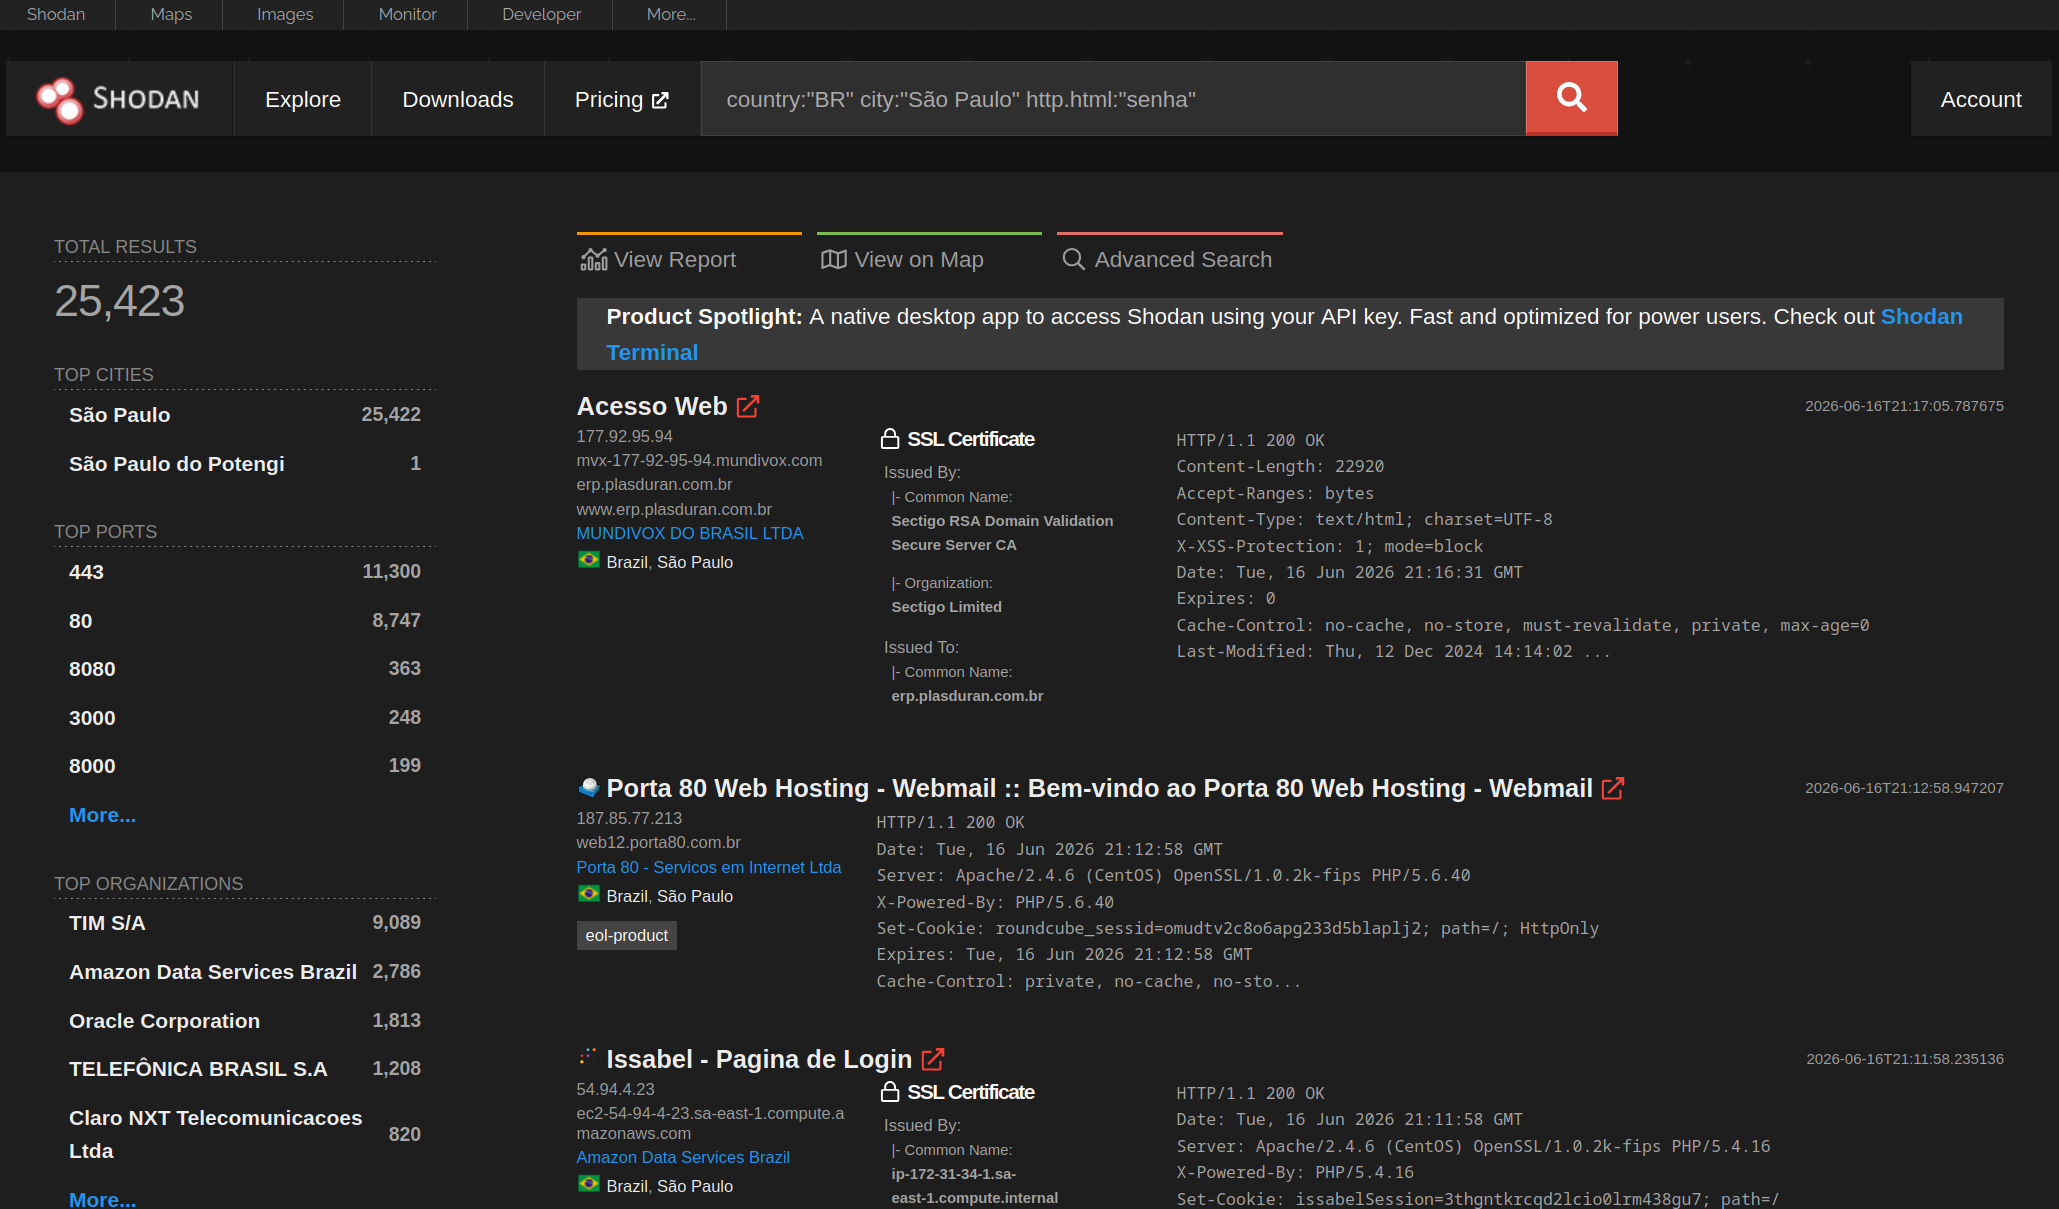
\includegraphics[width=0.95\textwidth]{./fig/atividade2-shodan.png}
\caption{Consulta realizada no Shodan utilizando filtros geográficos e conteúdo
HTML.}
\end{figure}

\paragraph{}
Os resultados permitiram identificar serviços web expostos que continham a
palavra ``senha'' em seu conteúdo, possibilitando a análise de informações
potencialmente sensíveis publicamente acessíveis.

\paragraph{}
Além dos conteúdos encontrados, o Shodan forneceu informações relevantes sobre
os ativos identificados, incluindo endereço IP, localização geográfica, portas
abertas, tecnologias detectadas e serviços em execução.

\paragraph{}
A atividade demonstrou como mecanismos de busca especializados podem ser
utilizados durante processos de OSINT para localizar informações expostas e
auxiliar atividades de reconhecimento e análise de segurança.
